%! Author = testpcfix
%! Date = 22/02/2023

% Preamble

% Packages

% Document
\pagebreak
\subsection{Ist-Zustand}\label{sec:ist-zustand}
\newglossaryentry{User Journey}{
    name=User Journey,
    description={User Journey ist ein Begriff aus der User Experience Design. User Journey ist ein Weg, den ein User durchläuft, um ein Ziel zu erreichen.}
}
\newglossaryentry{UserInterface}{
    name=UserInterface,
    description={UserInterface ist ein Begriff aus der User Experience Design. UserInterface ist die grafische Oberfläche, die ein User sieht und mit der er interagiert.}
}
Die Muttergesellschaft der DOOH media GmbH und einige Schwesterunternehmen nutzen Microsoft 365 und Office 365.
Diese Produkte sind sehr umfangreich und bieten viele Funktionen.
Die heutzutage gängige und weit verbreitete Terminplanung per Outlook oder Teams ist eines dieser Funktionen.
Diese Funktion ist nicht so praktikabel wie sie es sein könnte.
Vor allem nicht, wenn mehrere Unternehmen, das gleiche Gebäude und die gleiche Organisations-E-Mail besitzen.
Microsoft versucht so viele Nutzer wie möglich abzudecken und bietet vorzugsweise mehr Funktionen an, als weniger.
Dadurch ist die~\gls{User Journey}, also der Weg, den ein User durchläuft, um ein Ziel zu erreichen, sehr umständlich.
\newline
\newline
Falls ein User zufällig an einem Raum vorbeigeht oder vor einem Raum steht und sich fragt, ob dieser Raum belegt ist oder nicht, muss dieser erstmal Outlook oder Teams auf einem Gerät öffnen, zum Kalender des jeweiligen Raumes, falls er darauf überhaupt Zugriff hat und dann schauen, ob dieser Raum belegt ist oder nicht.
Dies ist umständlich und kann viel Zeit in Anspruch nehmen.


%\subsection{Definitionen}\label{subsec:definitionen}
%\begin{itemize}
%    \item \gls{RESTful}: RESTful ist ein Synonym für Representational State Transfer. RESTful ist ein Architekturstil für die Entwicklung von Webdiensten.
%    \item \gls{API}: API steht für Application Programming Interface. API ist eine Schnittstelle, die es einem erlaubt auf Daten zuzugreifen.
%    \item \gls{REST}: REST steht für Representational State Transfer. REST ist ein Architekturstil für die Entwicklung von Webdiensten.
%    \item \gls{HTTP}: HTTP steht für Hypertext Transfer Protocol. HTTP ist ein Protokoll, das es einem erlaubt auf Daten zuzugreifen.
%    \item \gls{JSON}: JSON steht für JavaScript Object Notation. JSON ist ein Datenformat, das es einem erlaubt Daten zu speichern und zu übertragen.
%    \item \gls{OAuth}: OAuth ist ein Protokoll, das es einem erlaubt sich mit einem Account anzumelden und somit auf Daten zuzug#
%    \item \gls{User Journey}: \gls{User Journey} ist ein Begriff aus der User Experience Design. \gls{User Journey} ist ein Weg, den ein User durchläuft, um ein Ziel zu erreichen.
%    \item \gls{UserInterface}: \gls{UserInterface} ist ein Begriff aus der User Experience Design. \gls{UserInterface} ist die grafische Oberfläche, die ein User sieht und mit der er interagiert.
%\end{itemize}
\pagebreak
\section{Soll-Zustand}\label{sec:soll-zustand}

\subsubsection{Anforderungen}\label{subsec:anforderungen}
Ein User soll am Bildschirm eines Tablets, welches vor dem Raum angebracht wird, erkennen können, ob dieser Raum belegt ist oder nicht.
Welche Termine am heutigen und nächsten Tag anstehen soll einfach ersichtlich sein.
Zudem möchte der Kunde einen Termin, am Gerät, vereinbaren können.
Der User soll also nicht mehr auf Outlook oder Teams angewiesen sein, sondern kann direkt am Bildschirm des Tablets sehen, ob der Raum belegt ist oder nicht.
Zudem soll der Raumstatus farbig dargestellt werden, sodass der User sofort erkennen kann, ob der Raum belegt ist oder nicht, sowohl am User Interface, als auch an den LED Strips des Tablets.
\subsubsection{User Interface}\label{subsec:user-interface}
Das User Interface soll, so gestaltet sein, dass der User sofort erkennen kann, ob der Raum belegt ist oder nicht.
Des Weiteren soll das \gls{UserInterface} so gestaltet sein, dass der User auch Termine für den Raum vereinbaren kann.
Dafür wird die Hintergrundfarbe des Containers, in dem der Raumstatus angezeigt wird, in Abhängigkeit vom Raumstatus, rot, gelb oder grün sein.
Falls der Termin gerade stattfindet, soll dieser rot dargestellt werden, falls er innerhalb der nächsten 15 Minuten stattfindet, soll er gelb dargestellt werden und falls er in der Zukunft stattfindet, soll er grün dargestellt werden.
Sollte am heutigen Tag kein Termin stattfinden, wird der Raumstatus weiterhin grün dargestellt, jedoch wird der Text \("\)Keine weiteren Termine für Heute\("\) angezeigt.
Das Userinterface soll also eine Übersicht über die Termine des Raumes und einen Button zum Vereinbaren eines Termins enthalten.
\newline
Hier ein Workflowdiagramm, welches den Ablauf der Terminbuchung beschreibt.
\par\vspace{1cm}
\centering
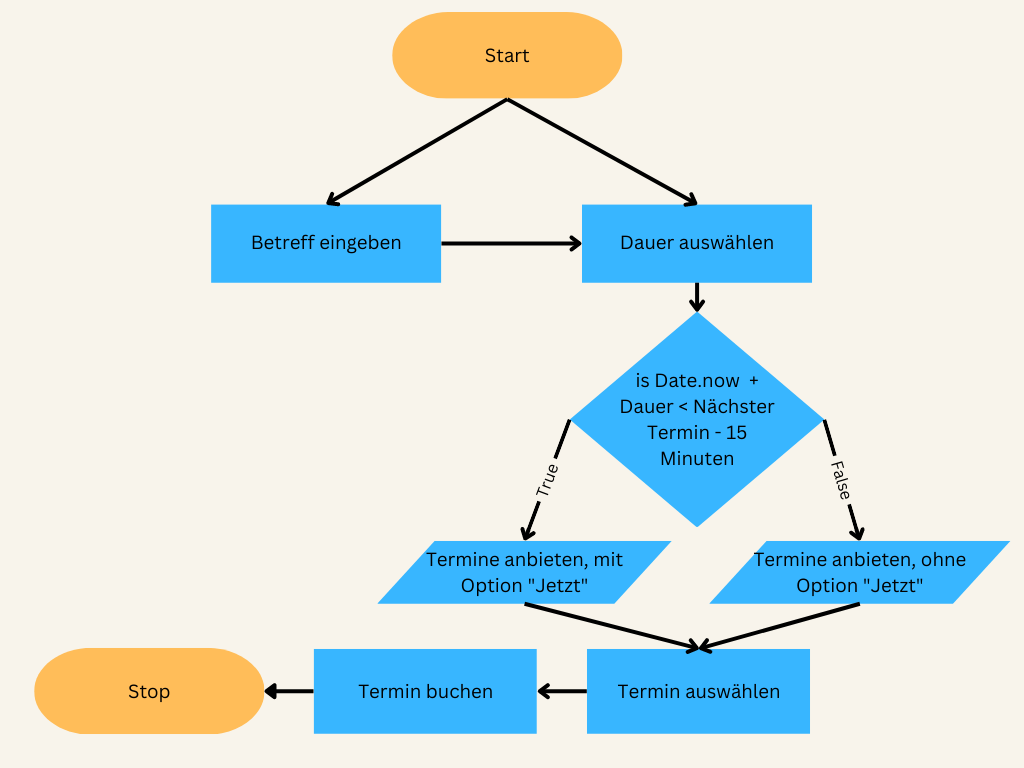
\includegraphics[width=0.8\textwidth]{Bilder/Workflow Terminbuchung}
\caption{Workflow Terminbuchung}
\label{fig:Workflow Terminbuchung}
\par\vspace{1cm}
\raggedright
\newline
Die Rechtecke stellen die einzelnen Schritte des Anwenders dar.
Pfeile zeigen den Ablauf des Anwenders.
Entscheidungen der Software werden durch die Pfeile mit einem Pfeilspitze dargestellt.
Falls diese Entscheidung zu einer Änderung der Daten führt, wird die Folge als Parallelogramm dargestellt.
\newline
\newline
Von den Grafikdesignerinnen unseres Unternehmens und der Muttergesellschaft wurde ein Design für das User Interface erstellt.

\newline
\par\vspace{1cm}
\centering
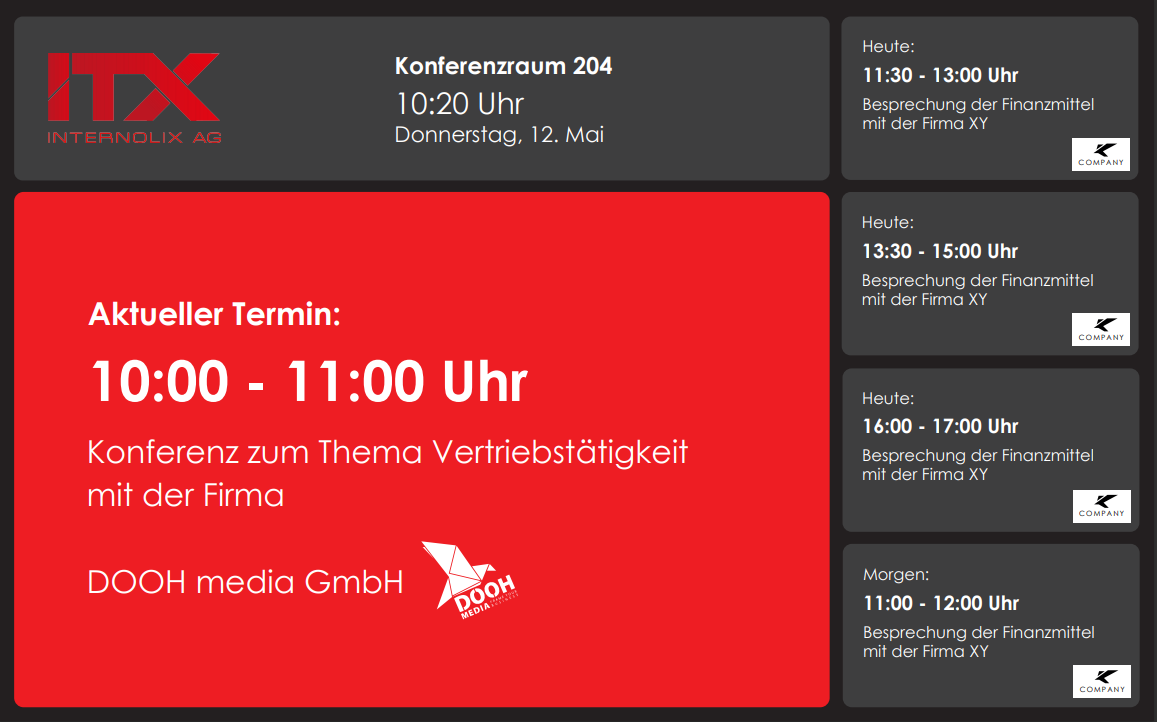
\includegraphics[width=0.8\textwidth]{Bilder/GrafikdesignerMockup}
\caption{GrafikdesignerMockup}
\label{fig:GrafikdesignerMockup}
\par\vspace{1cm}
\raggedright
Dieses Design, ist jedoch in seiner Ausführung nicht praktikabel.
Es wurden nicht die gängigen Konventionen für kontrastreiche Farben und Schriftarten berücksichtigt.
Beispielsweise sind die dunkelgrauen Boxen mit einem fast schwarzen Hintergrund der Seite und einem fast weißen Text nicht gut differenzierbar.
Des Weiteren wurde bei der Erstellung des Designs nicht genug auf die kleine Auflösung und Displaygröße des Tablets geachtet.
Dies sind alles Eigenschaften und Variablen, die bei der Gestaltung des Userinterface noch beachten sollte.
\newline
Das Design existiert, in sechs Versionen, die sich in darin unterscheiden, ob sie gerade im \("\)Dark Mode\("\) oder \("\)Light Mode\("\) sind und basierend auf ihrem Belegungsstatus, mit den Farben rot, gelb und grün.
\newline
\newglossaryentry{Responsive Design}{name={Responsive Design}, description={Responsive Design ist ein Begriff aus der User Experience Design. Responsive Design ist ein Design, das sich an die Größe des Bildschirms anpasst.}}

\gls{Responsive Design} wurde hier nur für das Format berücksichtigt, da die Anwendung nur für Tablets und Desktops im Landscape-Modus gedacht ist.
\newglossaryentry{DarkMode}{
    name=DarkMode,
    description={Dark Mode ist ein Begriff aus der User Experience Design. Dark Mode ist ein Modus, bei dem der Hintergrund dunkel ist und der Text hell.}
}
\newglossaryentry{LightMode}{
    name=LightMode,
    description={Light Mode ist ein Begriff aus der User Experience Design. Light Mode ist ein Modus, bei dem der Hintergrund hell ist und der Text dunkel.}
}
\newglossaryentry{Landscape}{
    name=Landscape,
    description={Landscape ist ein Begriff aus der User Experience Design. Landscape ist ein Modus, bei dem das Gerät horizontal liegt.}
}

\subsubsection{LED Strips}\label{subsec:led-strips}
\newglossaryentry{LED Strips}{
    name=LED Strips,
    description={LED Strips sind eine Art von LED Leuchtmittel. LED Strips sind in der Regel lang und dünn und werden in Streifen angebracht.}
}
Die~\gls{LED Strips} sollen in der Farbe leuchten, die dem Raumstatus entspricht.